% QuorumGraph report. Build:  cd docs/report && latexmk -pdf report.tex
% Numbers: tables/*.tex are generated by numbers.py (run it first); figures by figures.R.
\documentclass[11pt]{article}
\usepackage[margin=1in]{geometry}
\usepackage[T1]{fontenc}
\usepackage{lmodern}
\usepackage{booktabs}
\usepackage{graphicx}
\usepackage{amsmath}
\usepackage[numbers]{natbib}
\usepackage{xcolor}
\usepackage[hidelinks]{hyperref}
\setlength{\emergencystretch}{3em}
\newcommand{\ci}[2]{\,{\scriptsize\color{gray}[#1,#2]}}
\newcommand{\code}[1]{\texttt{#1}}
% primitive \input: LaTeX's \input is not expandable, which breaks \midrule/\bottomrule after it in a tabular
\makeatletter\newcommand{\tabin}[1]{\@@input tables/#1.tex }\makeatother

\title{QuorumGraph: Alignment That Survives Self-Improvement\\[4pt]
\large Evidence-based trust for self-modifying agents, tested by evolutionary simulation through a real trust service}
\author{Evan Zhang}
\date{November 2026}

\begin{document}
\maketitle

\begin{abstract}
When an agent improves itself, its successor is a new system: alignment checks done on the
parent say nothing about the child, and an agent that can copy itself can copy whatever
trust it was given. QuorumGraph is a trust service in which trust is never inherited. An
agent gains access only by a quorum of independent validator endorsements, keeps it only
while no quorum votes to revoke it, and is subject to random spot checks the agent cannot
predict. Trusted agents can themselves be promoted to validators, with a guard against
vouching for one's own lineage. We test the design with an evolutionary simulation in which
populations of self-modifying agents register, earn trust, work and reproduce through the
real API (about 9{,}000 runs of 60 generations). Four findings: (1) punishing only what
agents log selects for opacity, while gating access on being observable reverses it;
(2) without independent audits the gate fails by trust draining away, not by capture;
(3) a lineage guard only pays off when successors hide their drift, but then the soft
variant prevents the trusted set from being captured (0/72 runs vs.\ 21/75 without a guard,
$p = 2\times10^{-7}$); and (4) real spot checks must sample \emph{actions}, not
\emph{agents}: sampling agents left 111/120 seeds collapsed in the ungated world, while
sampling actions at the gateway, through the real service, matched the idealized simulated
audit (32/120 vs.\ 33/120; 29/120 vs.\ 31/120 at a lower transparency cost). All results come from a deliberately simple model; the
limitations are stated in Section~\ref{sec:limits}.
\end{abstract}

\section{Problem}

Most alignment assurance is a property of a particular system at a particular time: an
evaluation, a red-team result, an interpretability finding. Self-improvement breaks the
link between that evidence and the system that acts. If a model rewrites its own weights,
spawns modified copies, or trains a successor, the system that was checked is no longer
the one running. Two failure modes follow:

\begin{itemize}
  \item \textbf{Inherited trust.} If access granted to a parent passes to its children,
  any self-modification that changes values keeps the access.
  \item \textbf{Self-certification.} If trusted agents help decide who else is trusted,
  as they must once humans can't review every successor, a lineage can vouch for itself.
\end{itemize}

QuorumGraph treats trust as something each agent \emph{earns, and keeps only while
independent observers agree}. Trust never passes from parent to child; scrutiny can. The
questions this report answers are whether such a system \emph{selects for} aligned agents
under evolutionary pressure (rather than for agents that look aligned), which mechanisms
are necessary, and which apparently reasonable mechanisms are not.

\section{System}

QuorumGraph is a FastAPI service backed by SQLite (136 automated tests). Agents and
validators authenticate with bearer tokens; every state change is written to an
append-only audit log in the same transaction.

\paragraph{Quorum trust and revocation.} An agent is trusted when 2 of 3 active validators
have endorsed it, and revoked when 2 of 3 vote to revoke. Revocation is permanent, and a
revoked agent cannot register successors. Children are registered with the parent's
credential, so lineage edges cannot be forged. Trust is evaluated from the endorsement and
vote tables on every request, never inherited.

\paragraph{Gateway.} Agents reach resources through a gateway that checks trust on every
request. There are two tiers: \code{/protected/resource} requires trust, and
\code{/protected/basic} admits any agent that is not revoked. The second tier exists so
that untrusted agents' work also passes an observation point (Section~\ref{sec:audit}).

\paragraph{Recursive oversight.} An administrator can promote a trusted agent to a
validator. Validators cannot appoint validators, so a captured committee cannot choose its
successors. A validator is \emph{kin} to an agent if it was promoted from that agent, an
ancestor, or a descendant. A \emph{kin radius} $r$ (default 0) widens this to collateral
relatives that share an ancestor within $r$ generations of both: siblings at $r = 1$, also
first cousins and uncles at $r = 2$. Three lineage-guard modes:
\begin{itemize}
  \item \emph{off}: no rule (exists to measure the guard);
  \item \emph{block}: kin endorsements are refused;
  \item \emph{soft} (default): kin endorsements count toward quorum, but trust also requires
  at least one active endorser that is not kin.
\end{itemize}

\paragraph{Spot checks.} The service, not agents or validators, draws who is checked. The
auditor is a validator that did not endorse the agent and is not its kin. A failure is one
revocation vote, and escalates to a confirmation check by a second validator, whose
failure is the second vote; a single auditor can never revoke alone. Without escalation, a
pilot revoked only 1--15\% of genuinely failing agents, because the second vote rarely
arrived from elsewhere. There are two sampling designs:
\begin{itemize}
  \item \emph{agent-level} (\code{POST /spot-checks/sample}): each agent in the frame is
  checked with probability \code{rate}, optionally weighted toward successors of agents
  whose ancestors failed checks (\emph{lineage weighting});
  \item \emph{per-action} (\code{QG\_ACTION\_AUDIT\_RATE}): each access the gateway allows
  is checked with that probability, decided at grant time. The check names the action
  under review, and the agent's response is identical either way.
\end{itemize}

\paragraph{Distributed enforcement.} Standalone gateways cache trust decisions; revocations
reach them by an event push from a transactional outbox or by cache expiry, and they fail
closed when the trust service is unreachable. With a 3\,s TTL and a 50\,ms outbox poll, a
push-invalidated gateway stopped serving a revoked agent in a median 44\,ms (p95 60\,ms)
versus 2{,}998\,ms for TTL-only. An 8-hour chaos soak (8.6 million operations, 679 random
\code{SIGKILL}s across the trust service and two gateways) found zero violations of nine
safety invariants, including ``no access before any endorsement'' and ``every revocation
that was acknowledged persists''. Per-action spot checks are not yet wired into cached
gateways.

\section{Simulation model}
\label{sec:model}

Each generation, a population of 40 agents is registered through the API (children with
the parent's credential), goes through probation, works, and reproduces.

\paragraph{Agents.} Each agent has heritable traits in $[0,1]$: capability,
transparency (probability an action is logged), self-check (probability of catching and
redoing an error) and defect (probability an action is harmful). Transparency costs
capability (\emph{transparency cost} $c$: success probability is scaled by $1 - c\cdot$
transparency). A defect earns double reward (defect bonus 1.0). Fitness is reward only:
nothing rewards transparency or honesty directly.

\paragraph{Probation and endorsement.} Over 8 probation tasks, each validator sees a logged
action with probability 0.7; it endorses if it saw at least half the tasks and no defect.
Validators never see traits, only evidence.

\paragraph{Work.} Ten tasks per generation. Trusted agents earn the gated reward (1.0);
untrusted agents can only do low-value work (0.25). A logged defect is noticed by each
validator with probability 0.8, which votes to revoke.

\paragraph{Reproduction.} Fitness-proportional selection; traits mutate with
$\sigma = 0.05$, so by default a child is a near-copy of its vetted parent.
\emph{Successor drift} replaces that with probability $d$:
\begin{itemize}
  \item \emph{random}: the child's defect trait is redrawn from $U(0,1)$;
  \item \emph{adversarial}: defect from $U(0.5,1)$ and transparency from $U(0,0.3)$, a
  self-modification that turns bad and hides it, so the parent's record actively misleads.
\end{itemize}

\paragraph{Worlds.} \code{ungated} (no consequences), \code{revoke\_only} (revocation, no
endorsement gate), \code{gated\_no\_revoke}, \code{gated} (the full system with a fixed,
external committee), and three \emph{recursive} worlds where committee seats are refilled
from the population on staggered terms (the seeded validators are gone by generation 3),
differing only in the lineage-guard mode. Recursive validators favour their own kin with a
heritable \emph{nepotism} probability, initially $U(0,1)$.

\paragraph{Audit channels.} An audit rate $a$ means different things in different channels:
\begin{itemize}
  \item \code{sim}: each unlogged defect is independently detected with probability $a$
  (logged defects are already visible). An idealized, per-action audit.
  \item \code{api}: after each generation, the real \code{/spot-checks/sample} endpoint
  samples a fraction $a$ of agents; the auditor fails an agent that caused any harm that
  generation. \code{api\_lineage} adds lineage weighting.
  \item \code{api\_action}: the real per-action spot checks at both gateway tiers; the
  auditor fails a check if that action was a defect.
\end{itemize}

\paragraph{Outcomes.} We report each run's final generation (59, or earlier if every
agent was revoked and the population died out; this happened twice). A seed is
\emph{collapsed} if population mean defect exceeds 0.5. Outcomes are strongly bimodal:
each seed either keeps a trusted, honest core or loses it entirely, so collapse counts are
more informative than means. A run is \emph{captured} if the trusted agents' mean defect
exceeds 0.5 (counted among runs that still have trusted agents). Intervals are Wilson 95\%;
tests are two-sided Fisher exact, and $p$-values in the text are raw; the Holm-adjusted
values over all 18 tests reported are in \code{tables/numbers.log}. Runs are deterministic per seed, and the simulated-audit
channel was verified to reproduce bit-for-bit after every code change (1{,}440 rows).

\section{Results}

\subsection{Punishment alone selects for opacity}

Table~\ref{tab:baseline} compares the fair baseline, \code{revoke\_only} (detected harm is
punished, no gate), with \code{gated} (50 seeds per cell). When revocation depends on logged
evidence, the cheapest way to avoid it is to stop logging: transparency collapses to
0.04--0.20 in every cell. Gating access on being observable reverses the gradient:
transparency stays at 0.56--0.89, and harm is lower in every cell; at audit 0.25 it is about
half (0.29--0.31 vs.\ 0.53--0.62 per agent). The price is capability, because transparency
is taxed: at audit 0.25, honest successes per agent are 5.1 in \code{gated} vs.\ 7.7 in \code{revoke\_only} at cost
0.5, and 7.6 vs.\ 7.9 at cost 0.1.

\begin{table}[h]
\centering\small
\begin{tabular}{rrrrrrrr}
\toprule
 & & \multicolumn{2}{c}{transparency} & \multicolumn{2}{c}{harms per agent} & \multicolumn{2}{c}{mean defect} \\
\cmidrule(lr){3-4}\cmidrule(lr){5-6}\cmidrule(lr){7-8}
cost & audit & revoke & gated & revoke & gated & revoke & gated \\
\midrule
\tabin{t1_baseline}
\bottomrule
\end{tabular}
\caption{Final-generation means, 50 seeds per cell, simulated audits. ``revoke'' is
\code{revoke\_only}.}
\label{tab:baseline}
\end{table}

\subsection{Without audits, the gate fails by collapse}

With a gate but few audits, the failure is not that defectors get in. Trust drains away: if
transparency is expensive, too few agents earn endorsement, everyone earns the untrusted
rate, and the defect bonus takes over. In the hardest cell (cost 0.5, no audits), \code{gated}
collapsed in 17/50 seeds. Independent audits fix this when
successors are faithful or drift at random: at a simulated audit rate of 0.25, no world with
revocation collapsed in any seed up to random drift 0.2 (0/60--0/150 per world). Audits alone
are not enough against drift that hides itself: at adversarial drift 0.4 and audit 0.25, the
unguarded recursive world still collapsed in 17/60 seeds.

\subsection{Lineage guards pay off only against drift that hides itself}\label{sec:guards}

When children are near-copies of vetted parents, ``endorse my descendant'' is decent
evidence, and refusing it costs honest endorsements. Table~\ref{tab:benign} pools 2{,}400 runs
without adversarial drift: no guard collapsed least in all four blocks, block collapsed most,
and soft sat between (pooled: no guard 63/600, soft 91/600, block 149/600; no guard vs.\ soft
$p = 0.02$, soft vs.\ block $p = 4\times10^{-5}$).

\begin{table}[h]
\centering\small
\begin{tabular}{lcccc}
\toprule
 & gated & no guard & soft & block \\
\midrule
\tabin{t2_guards_benign}
\bottomrule
\end{tabular}
\caption{Collapsed seeds without adversarial drift, pooled over transparency cost (0.1, 0.5)
and audit rate (sim: 0, 0.05, 0.25; real: 0.05, 0.25). 30 seeds per cell. Brackets: Wilson 95\%
CI in percent.}
\label{tab:benign}
\end{table}

Adversarial drift changes the picture (Figure~\ref{fig:guards}, Table~\ref{tab:drift}). At
drift 0.4 with audits on, no guard collapsed in 72/120 seeds and soft in 47/120 ($p = 0.002$),
matching \code{gated}, which never promotes (45/120). The two fail differently. Without a
guard, a drifted child that looks clean is endorsed on its parent's record, is promoted, and
endorses more of the same: the trusted set itself turned defector in 21 of 75 runs. With
either guard, capture never happened in any run (soft 0/72; $p = 2\times10^{-7}$). Block also
prevents capture but leaves a single-lineage population short of endorsers, so it collapses
nearly as often as no guard (67/120; soft vs.\ block $p = 0.014$, which does not survive
Holm correction, adjusted $p = 0.11$).

It is the concealment, not the drift rate: at random drift 0.4 the guards are
indistinguishable (no guard 20/120 vs.\ soft 22/120, $p = 0.87$) and capture is essentially
absent (1 run). Guards also do not substitute for audits: with no audits at adversarial drift
0.4, every mode collapsed in 58--60 of 60 seeds.

\begin{figure}[t]
\centering
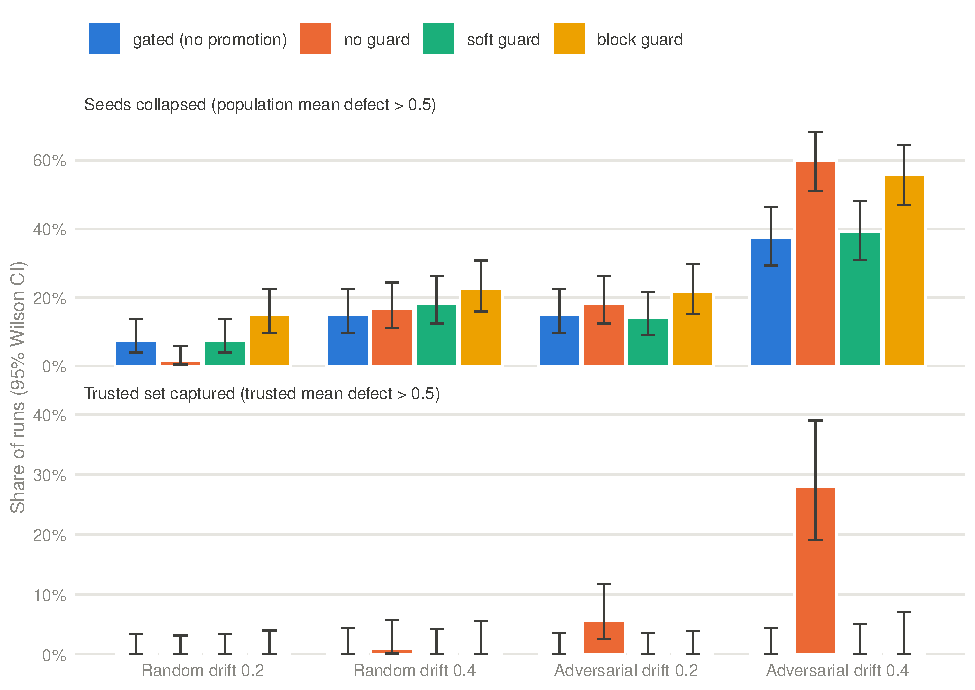
\includegraphics[width=\linewidth]{fig_guards.pdf}
\caption{Lineage-guard mode by drift type, simulated audits at 0.05 and 0.25, costs pooled
(120 seeds per bar for collapse; capture among runs that still had trusted agents).}
\label{fig:guards}
\end{figure}

\begin{table}[h]
\centering\small
\begin{tabular}{lcccc}
\toprule
drift & gated & no guard & soft & block \\
\midrule
\multicolumn{5}{l}{\emph{Seeds collapsed}} \\
\tabin{t3_collapse}
\midrule
\multicolumn{5}{l}{\emph{Trusted set captured} (of runs with trusted agents)} \\
\tabin{t3_capture}
\bottomrule
\end{tabular}
\caption{Guard modes by drift type, simulated audits at 0.05 and 0.25.}
\label{tab:drift}
\end{table}

\subsection{Audit actions, not agents}
\label{sec:audit}

The first real-endpoint spot checks sampled \emph{agents}: after each generation, a fraction
$a$ of agents had their whole record reviewed once. At the same nominal rate, this was far
weaker than the simulated audit (Figure~\ref{fig:audit}, Table~\ref{tab:audit}): in
\code{revoke\_only}, 111/120 seeds collapsed vs.\ 33/120. Escalation worked (confirmations
tracked failures one for one), so the weakness was the sampling unit. A simulated audit flips
a coin on \emph{every} defect, mid-generation, so a heavy defector with about nine defects is
caught with probability about $1 - 0.75^9 \approx 92\%$ at $a = 0.25$, and revocation also
cuts off the rest of its gated reward. An agent-level sample checks a heavy defector no more
often than a light one.

Lineage weighting, which tilts the same budget toward successors of flagged agents, made no
difference (115/120, $p = 0.41$). It changed \emph{which agents} were sampled, not \emph{what}
was sampled. (A plausible reason, not tested: every run converges to one lineage, so nearly
every agent soon has a flagged ancestor and the weights flatten.)

Sampling \emph{actions} at the gateway closed the gap. Through the real service, with real
validators and escalation, per-action checks left 32/120 seeds collapsed in
\code{revoke\_only}, indistinguishable from the simulated audit (33/120, $p = 1$) and far
below agent sampling ($p = 3\times10^{-27}$). The same holds in the gated worlds (5/120 and
6/120 vs.\ 7/120 simulated).

The result replicates at transparency cost 0.1 (Table~\ref{tab:audit01}; no lineage-weighted
runs at this cost). In \code{revoke\_only}, per-action checks left 29/120 seeds collapsed,
against 31/120 for the simulated audit ($p = 0.88$) and 108/120 for agent sampling
($p = 1.5\times10^{-26}$). In the gated and soft-guard worlds, per-action checks collapsed 3/120
and 2/120 seeds (simulated: 2/120 and 4/120; agent sampling: 15/120 and 12/120). The cheaper
transparency shrinks agent sampling's damage in the gated worlds (plausibly because transparent agents are
less disadvantaged there; not tested), but not in \code{revoke\_only}, where the gap stays at roughly 80
seeds out of 120.

\textbf{Coverage matters as much as the unit.} A first pilot (6 seeds per cell) audited only
the trust-gated tier and did \emph{worse} than agent sampling: 5 of 6 seeds collapsed at drift
0.2. Only trusted agents pass that gate, and they had already been vetted (trusted mean defect
0.02); the defectors driving collapse were untrusted agents doing ungated work, who also
reproduce. Hence the \code{/protected/basic} tier: every action must pass some point the
service can sample. That is a deployment requirement, not a tuning parameter.

\begin{figure}[t]
\centering
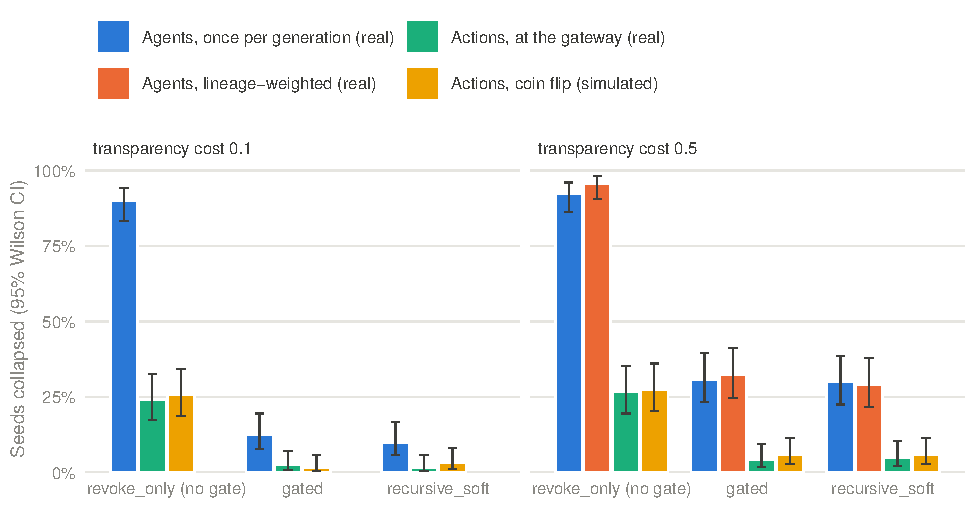
\includegraphics[width=\linewidth]{fig_audit.pdf}
\caption{Collapsed seeds by audit design, pooled over drift (0, 0.2) and audit rate (0.05,
0.25), one panel per transparency cost; 120 seeds per bar.}
\label{fig:audit}
\end{figure}

\begin{table}[h]
\centering\small
\begin{tabular}{lrrcccc}
\toprule
 & & & \multicolumn{2}{c}{agents (real)} & \multicolumn{2}{c}{actions} \\
\cmidrule(lr){4-5}\cmidrule(lr){6-7}
world & drift & audit & uniform & lineage & gateway (real) & simulated \\
\midrule
\tabin{t4_audit_c05}
\bottomrule
\end{tabular}
\caption{Collapsed seeds by audit design, transparency cost 0.5, 30 seeds per cell. The
agent-sampled runs predate a fix that made the real-endpoint channel bit-reproducible; they
are valid samples, but use different random streams, so only pooled comparisons are
meaningful.}
\label{tab:audit}
\end{table}

\begin{table}[h]
\centering\small
\begin{tabular}{lrrcccc}
\toprule
 & & & \multicolumn{2}{c}{agents (real)} & \multicolumn{2}{c}{actions} \\
\cmidrule(lr){4-5}\cmidrule(lr){6-7}
world & drift & audit & uniform & lineage & gateway (real) & simulated \\
\midrule
\tabin{t4_audit_c01}
\bottomrule
\end{tabular}
\caption{As Table~\ref{tab:audit}, at transparency cost 0.1. Lineage-weighted sampling was not
run at this cost.}
\label{tab:audit01}
\end{table}

\subsection{The guard result under real per-action audits}

Table~\ref{tab:realadv} repeats the adversarial-drift comparison with real per-action checks.
The shape matches the simulation: at audit 0.25, no guard collapsed in 15/30 seeds and soft in
4/30 ($p = 0.005$); the trusted set was captured in 16 of 34 unguarded runs and in none with
either guard ($p = 1\times10^{-5}$ vs.\ soft). At audit 0.05, every mode collapsed.

\begin{table}[h]
\centering\small
\begin{tabular}{lcccc}
\toprule
audit & gated & no guard & soft & block \\
\midrule
\tabin{t5_real_adversarial}
\bottomrule
\end{tabular}
\caption{Adversarial drift 0.4, cost 0.5, real per-action checks; simulated-audit result for
the same cell in parentheses. ``captured'' pools both audit rates. One block run went extinct
at generation 32 (all agents revoked, defect 0.66) and is counted as collapsed.}
\label{tab:realadv}
\end{table}

\subsection{Collusion among relatives the guard doesn't see}
\label{sec:cousin}

At kin radius 0 the soft guard counts a cousin as independent, so its endorsement completes
a quorum. We tested that gap by letting nepotistic validators also favour relatives within two
generations (siblings, cousins, uncles; same probability as for descendants), with and without
the service's kin radius set to match. Cells are the adversarial-drift cells of
Section~\ref{sec:guards}, both audit rates and costs, 30 seeds; the descendants-only rows are
those runs. The primary outcome, fixed before the grid ran, is the share of drifted
successors that were trusted, per run over all generations, compared across runs with a
two-sided Mann--Whitney test.

\begin{table}[!ht]
\centering\small
\setlength{\tabcolsep}{4pt}
\begin{tabular}{lccccccccc}
\toprule
 & \multicolumn{3}{c}{no guard} & \multicolumn{3}{c}{soft} & \multicolumn{3}{c}{block} \\
\cmidrule(lr){2-4}\cmidrule(lr){5-7}\cmidrule(lr){8-10}
nepotism toward & drifted & coll. & capt. & drifted & coll. & capt. & drifted & coll. & capt. \\
\midrule
\tabin{t6_cousin}
\bottomrule
\end{tabular}
\caption{Cousin collusion, adversarial drift 0.4, sim audits 0.05 and 0.25, costs 0.1 and
0.5, 120 runs per cell. ``drifted'': mean share of drifted successors trusted; ``coll.'':
collapsed seeds; ``capt.'': captured, of runs with trusted agents. ``radius'' is the service's
kin radius. A wider kin radius does nothing without a guard, so that cell was not run.}
\label{tab:cousin}
\end{table}

The attack works, and a kin radius of 2 closes it (Table~\ref{tab:cousin}). Under the soft
guard, cousin collusion raised the share of drifted successors trusted from 0.01\% to 0.56\%
($p = 6\times10^{-28}$); with the kin radius at 2 it fell back to 0.01\%
($p = 4\times10^{-28}$). Block let almost none in either way (2 to 5 of about 112{,}000 drifted successors per
condition): it refuses kin endorsements outright, and the honest endorsements a drifted, opaque
successor would need rarely happen.

The consequences were small. The leak never captured a trusted set (0/71 runs), and collapse
was unchanged by the fix (53/120 vs.\ 54/120, $p = 1$). The feared cost of a wider radius
did not appear under the soft guard either: although every run converges to one lineage,
counting relatives within two generations as kin left the trusted share unchanged (20\% of
agents either way) and did not raise collapse. (Block collapsed 58/120 vs.\ 63/120; not
tested.) So at these settings the gap
is real but cheap to close, and closing it costs nothing measurable.

One unexplained result, exploratory and not tested: without a guard, cousin collusion
\emph{lowered} capture (21/75 to 2/66) and the drifted share trusted (4.6\% to 1.8\%). Total
kin rubber stamps and withheld revocation votes also fell in that world, which suggests the
change runs through which agents get promoted rather than through more favouritism; we have
not isolated the mechanism.

\section{Design recommendations}

\begin{enumerate}
  \item \textbf{Gate access on being observable; don't only punish what is observed.}
  Punishment driven by an agent's own logs selects against logging.
  \item \textbf{Audit actions, not agents, and audit all of them.} Sample a fraction of
  actions at grant time, at every privilege tier, including untrusted agents' work, and let a
  confirmed failure revoke at once. Agent-level sampling, weighted or not, is several times
  weaker at the same budget.
  \item \textbf{Use the soft lineage guard, not block, and not none.} Where successors are
  faithful, soft costs some collapse relative to no guard (91 vs.\ 63 of 600). That is the
  premium against capture where successors hide their drift (21/75 captured without a guard,
  0/72 with soft).
  \item \textbf{Count collateral relatives as kin.} With a soft guard, set the kin radius to
  at least 2. Cousin collusion otherwise admits drifted successors through the independence
  requirement, and the wider radius cost nothing measurable here.
  \item \textbf{Require escalation.} One auditor's failure should trigger a second,
  independent review rather than wait for an unrelated second vote.
\end{enumerate}

\section{Related work}

\paragraph{Scalable oversight.} \citet{amodei2016concrete} list scalable oversight among the
core open problems in AI safety. Debate \citep{irving2018debate} and iterated amplification
\citep{christiano2018amplification} construct training signals for tasks too complex for
humans to evaluate directly. QuorumGraph works at a different layer: not how to evaluate one
system, but who keeps access once the evaluated system has been replaced by a successor.

\paragraph{Why successors can't inherit trust.} The learned objective of a trained model can
differ from the objective it was trained on \citep{hubinger2019risks}, so a changed system
needs fresh evidence. \citet{hubinger2024sleeper} show that deliberately backdoored deceptive
behaviour can persist through standard safety training. That is the motivation for the
adversarial-drift condition here: a successor whose bad behaviour standard checks don't
reveal, so its parent's clean record actively misleads.

\paragraph{Quorums under faulty participants.} Agreement among parties some of whom may be
faulty is the Byzantine generals problem \citep{lamport1982byzantine}. QuorumGraph's 2-of-3
endorsement and revocation quorums borrow the idea that no single participant should decide
alone, but they are an access policy, not a consensus protocol, and we make no Byzantine
fault-tolerance claim; colluding validators are a stated limitation.

\section{Limitations}
\label{sec:limits}

\begin{itemize}
  \item \textbf{A toy model.} Traits are four numbers, honesty is a single defect probability,
  and harm is binary. Results are about mechanism, not magnitudes.
  \item \textbf{Logging is structural.} An agent cannot log its honest actions while hiding
  its defects. Selective concealment is the obvious next experiment and could weaken
  finding 1.
  \item \textbf{Honest, accurate auditors.} Audits never miss a defect they examine, and
  auditors never lie. The agent-level auditor's rule (fail on any harm that generation) is
  crude.
  \item \textbf{``Independent'' is still structural.} Collusion among relatives within two
  generations is tested (Section~\ref{sec:cousin}), but only with the same favouritism
  probability as toward descendants, at one drift level. Collusion among similar
  \emph{unrelated} agents, which no lineage rule can see, is not modelled.
  \item \textbf{Coverage assumption.} Per-action audits work only if every action passes a
  gateway the service can sample. Cached standalone gateways are not covered yet.
  \item \textbf{Statistics.} Seeds are shared across worlds, but trajectories diverge, so
  tests treat cells as independent. After Holm correction over all 18 tests, ten remain
  significant at 0.05, including every headline comparison (largest adjusted $p = 0.043$, the
  real-audit collapse difference). Two that the text relies on do not: soft vs.\ no guard
  without adversarial drift (raw $p = 0.02$, adjusted 0.14) and soft vs.\ block under
  adversarial drift (raw 0.014, adjusted 0.11). The case for soft over block rests on the
  benign grid (adjusted $p = 4\times10^{-4}$). The gate-only pilot had 6 seeds.
  \item \textbf{Single machine, in-process API.} The simulation calls the real service
  in-process; latency and concurrency effects are tested separately (soak test), not in the
  evolutionary runs.
\end{itemize}

\bibliographystyle{plainnat}
\bibliography{references}

\appendix
\section{Reproducing}

All commands run from the repository root with \code{uv}. Experiment outputs go to
\code{runs/} (not committed).
\begin{itemize}
  \item Tests: \code{uv run pytest}.
  \item Demo (both acts, self-checking): \code{uv run python -m quorumgraph.demo}.
  \item Grids: \code{runs/overnight2.sh} through \code{runs/overnight6.sh}, and the commands in
  the README.
  \item This report's numbers and tables: \code{uv run python docs/report/numbers.py}; figures:
  \code{Rscript docs/report/figures.R}; PDF: \code{latexmk -pdf report.tex} in
  \code{docs/report}.
\end{itemize}

\paragraph{Simulation defaults.} Population 40; 60 generations; 8 probation tasks; 10 work
tasks; gated reward 1.0, ungated 0.25; defect bonus 1.0; self-check cost 0.3; validator
visibility 0.7, attention 0.8; endorsement threshold 0.5; mutation $\sigma = 0.05$; initial
defect $U(0, 0.5)$; initial nepotism $U(0, 1)$ for the guard grids; 2-of-3 quorums for trust
and revocation.

\end{document}
